%Introduction (Introducing the topic)

%AM: What is the problem?
%introduce the need to scale to multiple agile teams
Agile approaches are popular in software development for numerous reasons.
However, the structure of the agile process does not lend itself to large teams and is not suitable for large projects.
With the growth in complex software, situations arise where multiple agile teams need to work together to achieve a common goal.
%thesis statement
When scaling to parallel agile teams, the most important consideration is quality communication, both personal and architectural.
%
For an example of a company developing a complex piece of software, consider Spotify AB who has over 30 teams \cite{kniberg12}.
Spotify is a streaming music client which supports media, commercial, and social features.
The basic element of development organization at Spotify is the Squad, analogous to a Scrum team.
%Each Squad is the autonomous developer, with a localized working area, of a particular sub-system in the product.
Squads in related areas are grouped together into Tribes. 
The overall structure is illustrated in Figure~\ref{fig:spotify_structure}.
\begin{figure}[h]
  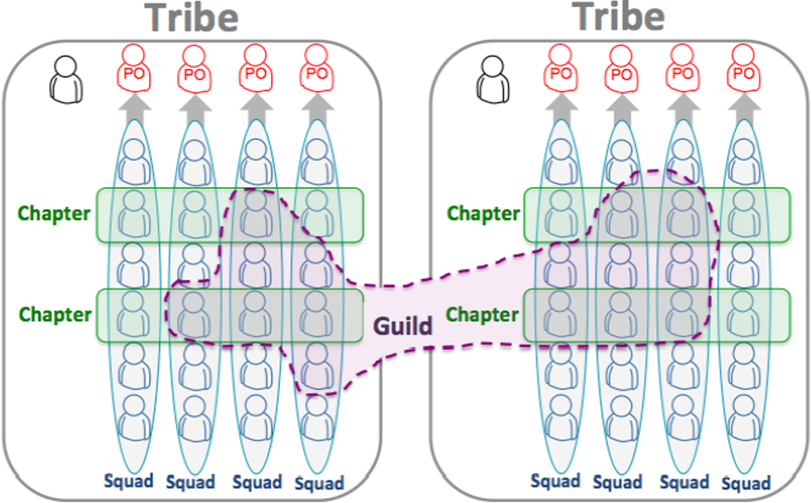
\includegraphics[width=\linewidth]{images/kniberg12_structure.png}
  \caption{Agile team organization at Spotify \cite{kniberg12}.}
  \label{fig:spotify_structure}
\end{figure}


%AM: Why is it interesting/important?
%introduce agile
As outlined in the Agile Manifesto \cite{beck2001agile}, an agile process gives individuals and interactions value over processes and tools.
An agile team should contain all that is required for them to do their work, thus interactions are intensely intra-team.
However, diverse feature sets such as required in the Spotify application necessitate many skillsets and substantial manpower.
By moving to a multi-team model, complex projects can benefit from agility, provided that the process is adapted.
%personal communication
Multiple teams increases the importance of communication, from simple interpersonal communication to system specification. 
The agile approach of interacting in-person can fail due to reasons such as the vertical structure of the company organization and layers of middle managers \cite{dzone_article}.
The large number of intermediaries can cause an agile process to breakdown as it takes longer than usual time for messages to reach their destination than can afforded.
%arch communication
In an agile process, where Big Design Up-front may typically be avoided, the move to multiple teams motivates a need to communicate design decisions.
%todo: component boundaries?
For successful integration of technological components, system elements must have well defined functional specifications, and interfaces.

%RA: feel like we can skip AM suggest section on Why is it hard.
%AM: What are the key components of [the] proposed approach? Also include assumptions/limitations
%We discuss approaches, which if implemented correctly, provide a more robust and functional process for inter-team agile development. 

%outline of rest of paper
This document is organized as follows: Introduction, Communication Concerns, Supporting Communication in Inter-team Development, and Conclusion. 
In Section ~\ref{sec:spt_ex}, we discuss example communication concerns in an agile project.
In Section ~\ref{sec:prop_appro}, we present some process adaptations that can help to resolve issues.
Lastly, Section ~\ref{sec:conclusion} concludes with an overview of important aspects of inter-team agile development.


%This problem is difficult to fix as this is so embedded in the working agile culture of the current organizations that changing them will take a long time, thus an immediate patch that works is required. %RA: this is an important observation, just too detailed for intro.